\documentclass[12pt,letterpaper]{article}
\usepackage[utf8]{inputenc}
\usepackage[spanish]{babel}
\usepackage[a4paper,margin=2.5cm]{geometry}
\usepackage{amsmath}
\usepackage{graphicx}
\usepackage{booktabs}
\usepackage{hyperref}
\usepackage{microtype}
\usepackage{array}
\usepackage{multirow}
\usepackage{enumitem}
\usepackage{setspace}
\graphicspath{
    {../../sprint_01/informes/figures/}
    {../../sprint_02/informes/figures/}
    {../../sprint_03/informes/figures/}
    {../../figures/}
}

\hypersetup{
    colorlinks=true,
    linkcolor=black,
    urlcolor=blue,
    pdftitle={Reporte Final Unificado Extendido - Proyecto Olist},
    pdfauthor={Marcelo de la Quintana, Gaston Nina, Gerick Toro}
}

\setstretch{1.12}

\begin{document}

\begin{titlepage}
    \centering
    {\Large Universidad Mayor de San Andres\par}
    \vspace{0.4cm}
    {\large Maestria en Inteligencia Artificial y Ciencia de Datos\par}
    \vspace{1.2cm}
    {\Huge \textbf{Reporte Final Unificado Extendido}\par}
    \vspace{0.4cm}
    {\Large Segmentacion Predictiva de Clientes Premium en Olist\par}
    \vspace{1.2cm}
    {\large Modulo de Implementacion de Soluciones de Inteligencia Artificial\par}
    \vspace{1.2cm}
    {\large
        Marcelo de la Quintana\par
        Gaston Nina\par
        Gerick Toro\par
    }
    \vfill
    {\large Junio 2026\par}
\end{titlepage}

\tableofcontents
\newpage

\section{Resumen Ejecutivo}
Este informe presenta una version integrada y desarrollada del proyecto de identificacion de clientes premium sobre Olist. El trabajo cubre la cadena completa de valor analitico: comprension del problema de negocio, auditoria de calidad de datos, definicion del target, construccion de un pipeline reproducible, entrenamiento supervisado, seleccion del modelo final, despliegue de un MVP y definicion de criterios de monitoreo y gobernanza.

El problema central consistio en identificar clientes de alto valor en una plataforma donde la mayor parte de la poblacion presenta una sola compra, lo que reduce la utilidad de variables tradicionales de recurrencia. A partir de este hallazgo se definio un target binario \textit{is\_premium}, calculado con el percentil 80 del gasto acumulado sobre pedidos entregados y congelado en BRL \textbf{197.01}. Esta definicion produce un segmento premium del \textbf{20\%} de los clientes que concentra el \textbf{56.03\%} de la facturacion, con un ticket promedio \textbf{4.36 veces} superior al regular.

El baseline inicial de regresion logistica obtuvo un ROC-AUC de \textbf{0.5355}, validando que el problema no podia resolverse con un esquema basico de variables RFMT. La construccion de nuevas variables operativas, logisticas, geograficas, de categoria y de comportamiento de pago permitio elevar el rendimiento hasta un ROC-AUC de \textbf{0.7929} y Gini de \textbf{0.5858}. Posteriormente, un benchmark de cinco algoritmos y una optimizacion de hiperparametros con Optuna consolidaron a LightGBM como modelo final, con ROC-AUC de validacion \textbf{0.8081}, Gini \textbf{0.6162} y umbral de decision \textbf{0.55}.

Finalmente, el modelo se integro en un MVP funcional con dashboard en Streamlit y API en FastAPI, ambos apoyados en el mismo artefacto serializado. En una simulacion de negocio, la estrategia focalizada mejoro el ROI desde \textbf{-89.57\%} en una campana masiva hasta \textbf{+250.40\%}. El informe cierra con lineamientos de privacidad, sesgo, monitoreo y reentrenamiento para sostener la utilidad del modelo frente a cambios del mercado.

\section{Introduccion}
La segmentacion de clientes de alto valor es una practica comun en marketing analitico, pero su efectividad depende de la calidad de la definicion del segmento y del poder real de las variables disponibles. En plataformas de comercio electronico es frecuente asumir que los clientes mas valiosos son tambien los mas recurrentes, pero esa hipotesis no siempre se sostiene. El caso Olist presenta precisamente ese desafio: una gran parte de la base realiza una sola compra, y dentro de esa misma estructura aparecen clientes que concentran valor por el monto de una transaccion, no por su repeticion.

El objetivo de este proyecto fue desarrollar un sistema predictivo que permitiera identificar clientes premium a nivel \texttt{customer\_unique\_id} usando informacion historica disponible en el ecosistema de Olist. El sistema debia ser tecnicamente reproducible, defendible desde negocio y suficientemente interpretable para integrarse en una demostracion funcional.

Para cumplir este objetivo se siguio una estrategia incremental:
\begin{enumerate}[label=\arabic*.]
    \item perfilar datos crudos y entender sus limitaciones;
    \item definir y defender un target premium estadistica y comercialmente consistente;
    \item convertir notebooks exploratorios en un pipeline reproducible;
    \item enriquecer el espacio de variables para resolver la baja capacidad del baseline;
    \item comparar algoritmos y seleccionar un modelo final;
    \item desplegar un MVP con explicabilidad y simulacion financiera;
    \item proponer criterios de gobernanza, monitoreo y reentrenamiento.
\end{enumerate}

\section{Problema de Negocio y Objetivo Analitico}
Olist opera como un integrador de vendedores dentro del comercio electronico brasileno. En este contexto, identificar clientes con alta probabilidad de pertenecer al segmento premium tiene implicaciones directas sobre:
\begin{itemize}
    \item asignacion de presupuesto comercial,
    \item priorizacion de campanas de retencion,
    \item venta cruzada sobre categorias de alto valor,
    \item reduccion de desperdicio en estrategias masivas.
\end{itemize}

El objetivo analitico no fue predecir compras futuras en sentido causal estricto, sino construir un scoring operativo que distinguiera a los clientes con mayor afinidad al segmento premium en funcion de sus patrones historicos observados.

La hipotesis inicial de trabajo era que el valor premium podria inferirse desde frecuencia, recencia, calificaciones, comportamiento de pago y logistica. Sin embargo, el propio analisis de datos mostro que la frecuencia pura era un discriminador mucho menos potente de lo esperado, obligando a una reformulacion del enfoque.

\section{Datos y Perfilado de Calidad}
El proyecto utilizo siete datasets crudos: clientes, ordenes, pagos, resenas, productos, vendedores e items de compra. El perfilado inicial tuvo dos objetivos: evaluar consistencia fisica y temporal, y entender si la estructura del negocio apoyaba o no la intuicion del target premium.

\subsection{Valores faltantes e inconsistencias}
Se detectaron nulos significativos en campos de texto de resenas y en algunas fechas logisticas, pero la principal alerta provino de inconsistencias cronologicas dentro del ciclo de vida de las ordenes. Entre los casos observados estuvieron:
\begin{itemize}
    \item entregas al transportista antes de la aprobacion del pago,
    \item registros de recepcion por parte del cliente anteriores a la etapa logistica,
    \item discrepancias entre fechas de compra, aprobacion y entrega.
\end{itemize}

Estas observaciones no invalidan el dataset, pero justifican reglas de saneamiento y cautela al disenar variables temporales.

\subsection{Asimetria monetaria y cola larga}
El gasto acumulado por cliente presento una distribucion marcadamente asimetrica, con \textit{skewness} aproximada de \textbf{7.92}. Esta propiedad hizo poco recomendable definir segmentos con promedios o umbrales sensibles a valores extremos. Por ello, el uso de percentiles robustos resulto metodologicamente mas apropiado.

\begin{figure}[h]
    \centering
    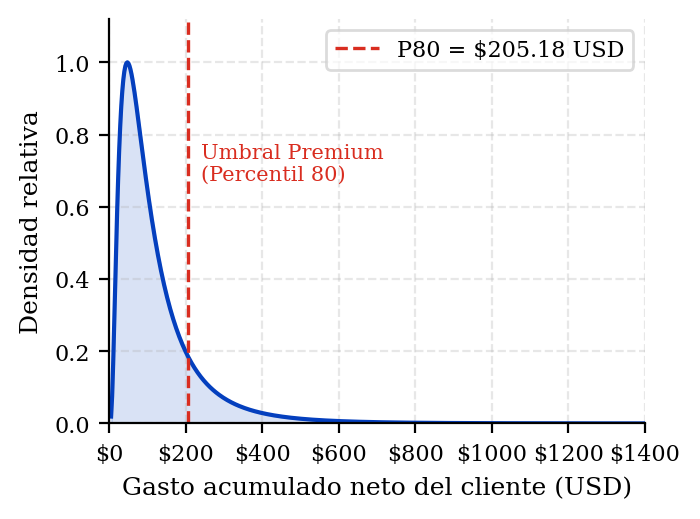
\includegraphics[width=0.85\textwidth]{fig_long_tail.png}
    \caption{Distribucion del gasto acumulado neto por cliente. La cola larga justifica una segmentacion basada en percentiles robustos.}
    \label{fig:ext_long_tail}
\end{figure}

\subsection{La paradoja del target}
El hallazgo mas importante del perfilado fue que aproximadamente el \textbf{97\%} de los clientes tenia solo una orden. Este hecho altera la intuicion habitual de CRM: los clientes premium en Olist no necesariamente son mas recurrentes, sino que muchas veces se distinguen por una compra unica de alto valor. Este comportamiento fue denominado internamente \textbf{Paradoja del Target} y se convirtio en el eje conceptual de todo el modelado posterior.

\section{Definicion del Target Premium}
La variable objetivo se definio sobre el gasto acumulado de pedidos con estado \texttt{delivered}. El target final fue:
\begin{equation}
is\_premium =
\begin{cases}
1 & \text{si } total\_spent \geq P80_{dev} = 197.01 \\
0 & \text{en caso contrario}
\end{cases}
\end{equation}

La decision de usar el percentil 80 respondio a criterios tecnicos y de negocio:
\begin{itemize}
    \item conserva una proporcion premium cercana al 20\%;
    \item evita un segmento excesivamente amplio o demasiado estrecho;
    \item se adapta mejor a la asimetria del gasto;
    \item es interpretable desde negocio como una segmentacion de alto valor.
\end{itemize}

Tambien se decidio congelar el umbral sobre el conjunto de desarrollo. De este modo, el target no cambia en cada corrida y las comparaciones entre experimentos permanecen consistentes.

\begin{table}[h]
\centering
\caption{Resumen del Target Premium}
\label{tab:ext_target}
\begin{tabular}{lr}
\toprule
Indicador & Valor \\
\midrule
Clientes totales & 96,096 \\
Clientes premium & 19,220 \\
Proporcion premium & 20.00\% \\
Umbral P80 congelado & BRL 197.01 \\
\bottomrule
\end{tabular}
\end{table}

\section{Validacion del Segmento desde Negocio}
Una definicion de target solo es defendible si produce un segmento economicamente relevante. En este caso, la validacion de negocio fue clara: el 20\% premium concentra el \textbf{56.03\%} de la facturacion, con un ticket promedio de BRL \textbf{402.66} frente a BRL \textbf{92.27} del segmento regular.

\begin{table}[h]
\centering
\caption{KPIs de Negocio por Segmento}
\label{tab:ext_kpis}
\begin{tabular}{lrr}
\toprule
Indicador & Premium & Regular \\
\midrule
Clientes & 19,220 & 76,876 \\
Participacion base & 20.00\% & 80.00\% \\
Facturacion & BRL 8,088,731.72 & BRL 6,348,315.77 \\
Participacion facturacion & 56.03\% & 43.97\% \\
Ticket promedio & BRL 402.66 & BRL 92.27 \\
\bottomrule
\end{tabular}
\end{table}

Estos resultados sostienen que el target no es una construccion arbitraria. El segmento detectado tiene sentido comercial y justifica el esfuerzo de clasificacion.

\section{Arquitectura del Pipeline Reproducible}
Una de las prioridades del proyecto fue convertir el trabajo exploratorio inicial en un pipeline modular y reutilizable. La arquitectura final quedo estructurada en cuatro pasos:
\begin{enumerate}[label=\arabic*.]
    \item \texttt{src/data/build\_master\_table.py}
    \item \texttt{src/features/build\_rfm\_features.py}
    \item \texttt{src/features/feature\_selection\_experiments.py}
    \item \texttt{src/models/evaluate\_model.py}
\end{enumerate}

Este diseno ofrece varias ventajas:
\begin{itemize}
    \item separacion clara entre construccion de datos, creacion de variables y modelado;
    \item persistencia de artefactos intermedios;
    \item trazabilidad de cada etapa;
    \item reuso del mismo flujo sobre desarrollo, validacion y backtest.
\end{itemize}

La master table final se consolido a nivel de \texttt{customer\_unique\_id} y quedo libre de duplicados. Sobre ella se construyeron 18 variables derivadas adicionales.

\section{Ingenieria de Variables}
Para superar la limitacion del baseline inicial se enriquecio el espacio de variables con cuatro grandes familias:
\begin{itemize}
    \item \textbf{Composicion del pedido:} intensidad y diversidad de items;
    \item \textbf{Pago y financiamiento:} cuotas, metodos y complejidad de pago;
    \item \textbf{Logistica y servicio:} retrasos, cancelaciones, brechas de entrega;
    \item \textbf{Contexto geografico y de categoria:} region, categoria principal y categorias de alto valor.
\end{itemize}

Entre las variables mas relevantes estuvieron \texttt{installments\_gt\_1\_flag}, \texttt{credit\_card\_flag}, \texttt{delivery\_gap}, \texttt{far\_region\_flag}, \texttt{top\_category\_group} y \texttt{top\_category\_is\_high\_value}.

El control de leakage se mantuvo como restriccion permanente. No se permitieron variables que reconstruyeran directamente el gasto objetivo ni identificadores operativos que inflaran artificialmente el poder predictivo.

\section{Seleccion Experimental de Variables}
La seleccion final no se hizo por criterio manual, sino mediante ocho experimentos reproducibles. El corte temporal oficial de evaluacion fue \textbf{2018-07-01}, separando entrenamiento y validacion de forma cronologica.

El experimento ganador fue \texttt{corr\_le\_0.85}, con \textbf{28 variables}. Su ventaja no fue solo el mejor equilibrio de desempeno, sino tambien la mayor parsimonia frente a sets mas grandes con ganancia marginal en AUC.

\begin{figure}[h]
    \centering
    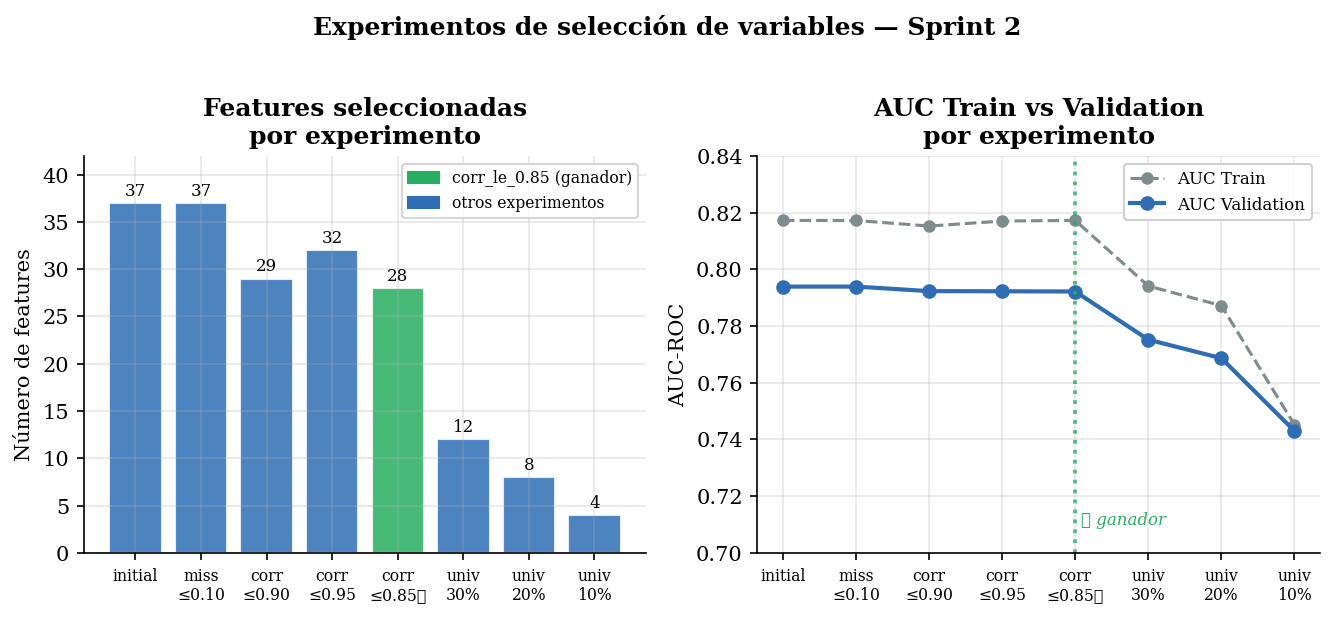
\includegraphics[width=0.88\textwidth]{fig_feature_selection.png}
    \caption{Comparacion de experimentos de seleccion de variables. El set final retiene alta capacidad predictiva con menor redundancia.}
    \label{fig:ext_feature_selection}
\end{figure}

\section{Baseline y Mejora del Desempeno}
El baseline inicial fue una regresion logistica con ponderacion balanceada de clases. Su desempeno fue:
\begin{itemize}
    \item Precision: 0.30
    \item Recall: 0.16
    \item F1-Score: 0.21
    \item ROC-AUC: 0.5355
\end{itemize}

Lejos de ser un fracaso, este resultado fue diagnostico: confirmo que las variables basicas no eran suficientes para capturar el segmento premium dentro de la estructura de Olist.

Al incorporar las nuevas variables y el set final seleccionado, el modelo de referencia del pipeline alcanzo:
\begin{itemize}
    \item Precision: 0.4766
    \item Recall: 0.6294
    \item F1-Score: 0.5424
    \item ROC-AUC: 0.7929
    \item Gini: 0.5858
\end{itemize}

\begin{table}[h]
\centering
\caption{Comparacion de Metricas: Baseline vs. Pipeline Enriquecido}
\label{tab:ext_metrics}
\begin{tabular}{lrr}
\toprule
Metrica & Baseline & Pipeline enriquecido \\
\midrule
Precision & 0.3000 & 0.4766 \\
Recall & 0.1600 & 0.6294 \\
F1-Score & 0.2100 & 0.5424 \\
ROC-AUC & 0.5355 & 0.7929 \\
Gini & 0.0710 & 0.5858 \\
\bottomrule
\end{tabular}
\end{table}

\begin{figure}[h]
    \centering
    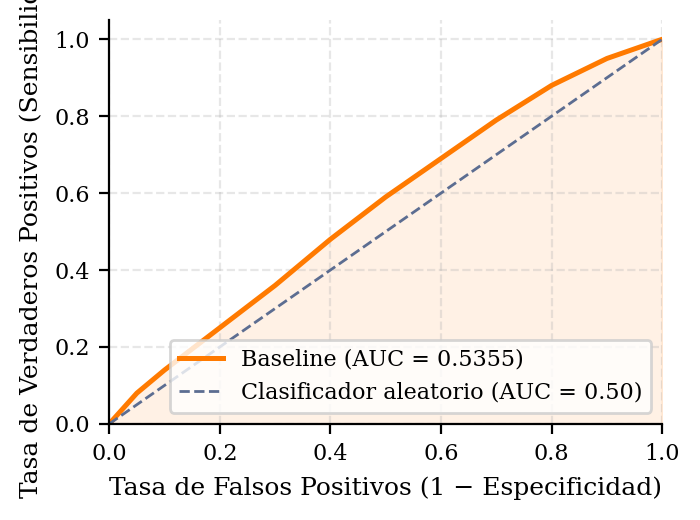
\includegraphics[width=0.82\textwidth]{fig_roc_baseline.png}
    \caption{Curva ROC del baseline. Su cercania al azar justifico la necesidad de enriquecer el espacio de variables.}
    \label{fig:ext_roc_base}
\end{figure}

\section{Benchmark de Modelos y Seleccion del Ganador}
Una vez estabilizado el pipeline, se compararon cinco modelos candidatos:
\begin{enumerate}[label=\arabic*.]
    \item Regresion Logistica
    \item Random Forest
    \item Gradient Boosting
    \item XGBoost
    \item LightGBM
\end{enumerate}

Los criterios de comparacion incluyeron ROC-AUC, Gini, F1, Recall y gap de sobreajuste. Este punto es importante: no se selecciono el modelo solo por AUC. En un contexto de negocio, dejar de detectar clientes premium tiene un costo alto, por lo que el Recall y el F1 debian influir en la decision.

LightGBM y XGBoost quedaron como finalistas. Luego se aplico Optuna TPE con 50 \textit{trials} por modelo. LightGBM se consolido como ganador por liderar las metricas de discriminacion global con estabilidad razonable.

\begin{table}[h]
\centering
\caption{Resultado del Modelo Final}
\label{tab:ext_final_model}
\begin{tabular}{lr}
\toprule
Indicador & Valor \\
\midrule
Modelo final & LightGBM tuneado \\
ROC-AUC validacion & 0.8081 \\
Gini validacion & 0.6162 \\
Umbral operativo & 0.55 \\
\bottomrule
\end{tabular}
\end{table}

\begin{figure}[h]
    \centering
    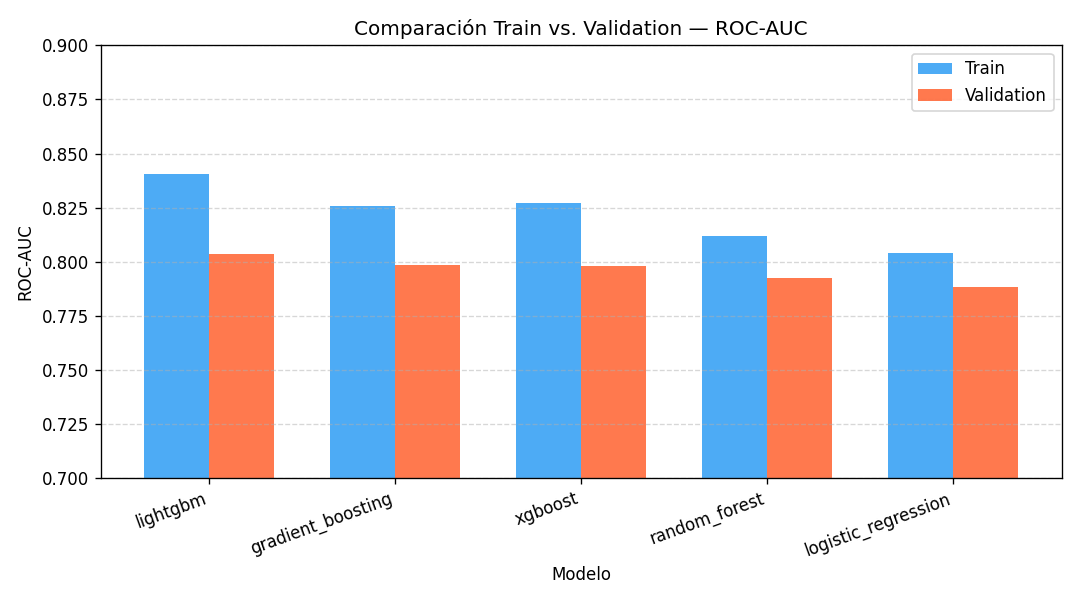
\includegraphics[width=0.82\textwidth]{fig_benchmark_auc.png}
    \caption{Benchmark de modelos candidatos. LightGBM y XGBoost dominaron el ranking final.}
    \label{fig:ext_benchmark}
\end{figure}

\section{Serializacion y MVP}
El modelo final fue serializado como \texttt{modelo\_final.pkl}. Sobre este artefacto se construyo un MVP con dos capas:
\begin{itemize}
    \item un dashboard en Streamlit para exploracion, scoring y explicacion visual;
    \item una API en FastAPI para inferencia estructurada.
\end{itemize}

Ambas superficies consumen el mismo modelo y el mismo esquema de variables. Esta consistencia fue una condicion clave para la trazabilidad tecnica del proyecto.

\begin{figure}[h]
    \centering
    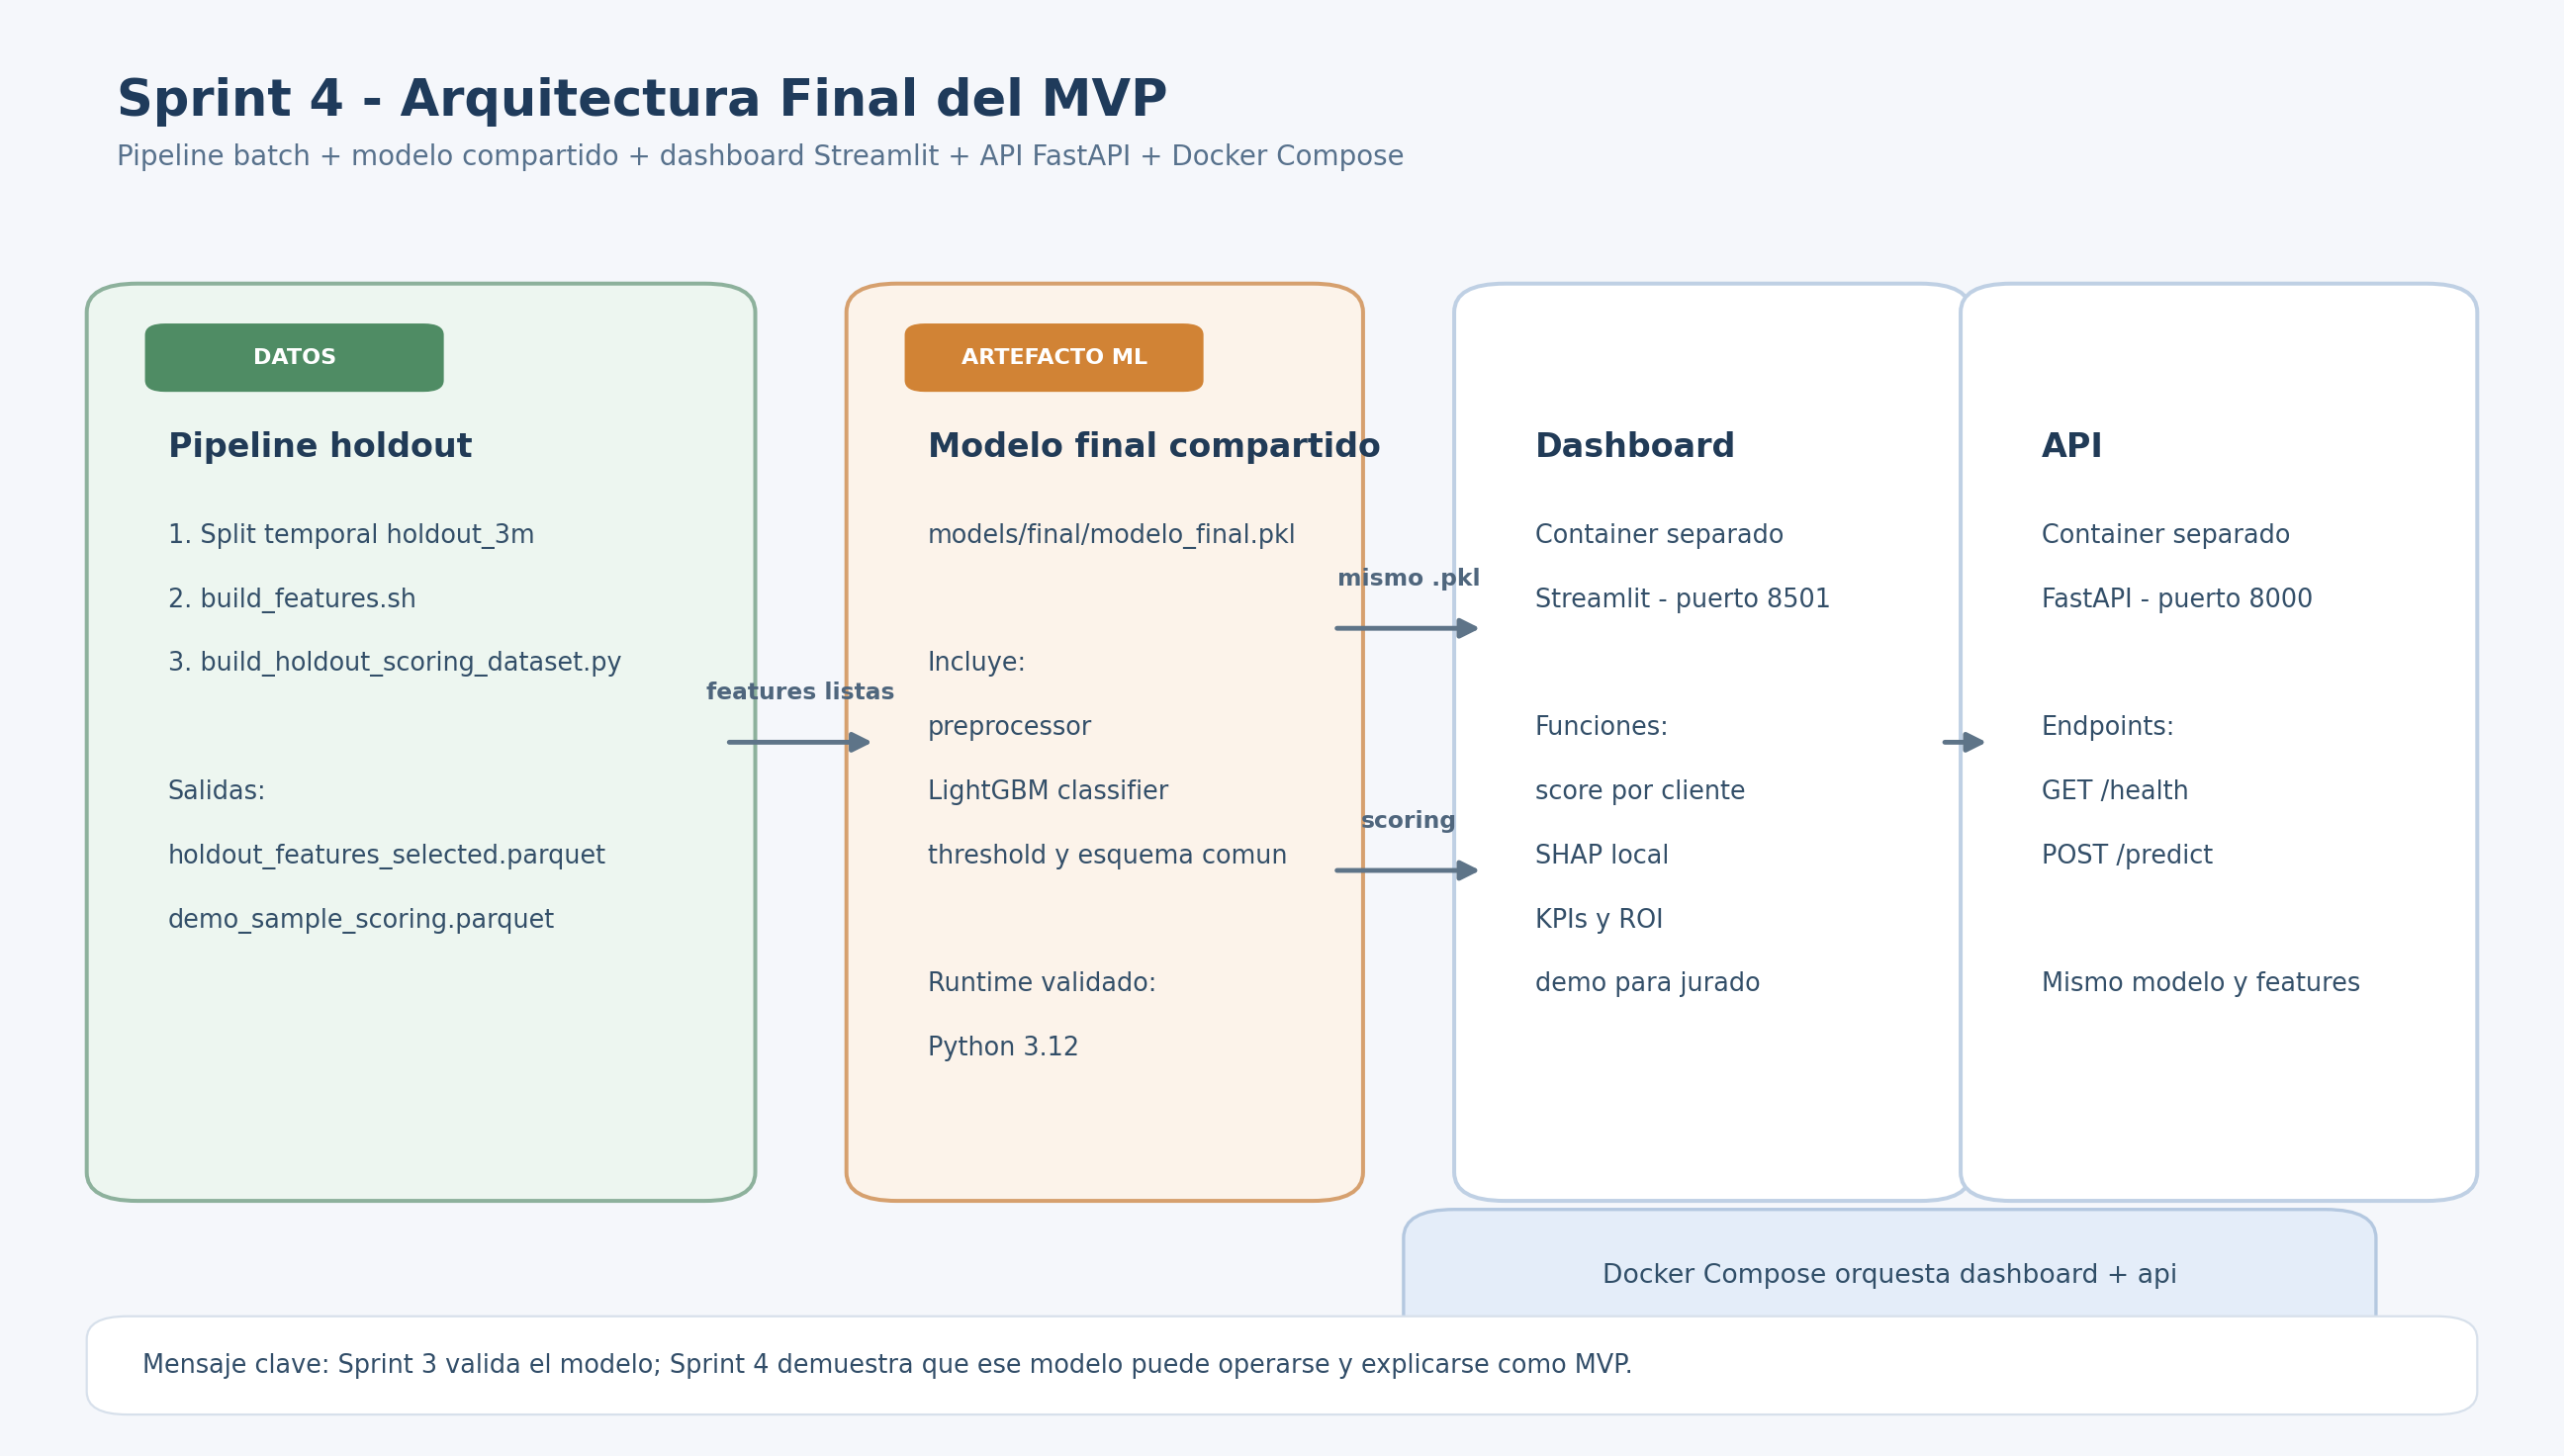
\includegraphics[width=0.88\textwidth]{sprint_04_mvp_architecture.png}
    \caption{Arquitectura del MVP. El pipeline prepara el dataset y tanto dashboard como API reutilizan el mismo artefacto del modelo.}
    \label{fig:ext_mvp}
\end{figure}

\section{Validacion Backtest e Interpretacion Correcta}
La validacion final del MVP se hizo sobre un backtest formal de agosto de 2018. El split tecnico historico \texttt{holdout\_3m} se conserva por trazabilidad, pero septiembre y octubre solo aportan 20 ordenes combinadas y no constituyen una base seria para evaluacion final. Las metricas observadas sobre el backtest fueron:
\begin{itemize}
    \item ROC-AUC: 0.9876
    \item Gini: 0.9751
    \item Precision: 43.80\%
    \item Recall: 56.11\%
    \item F1-Score: 49.20\%
\end{itemize}

\begin{table}[h]
\centering
\caption{Metricas Tecnicas sobre Backtest}
\label{tab:ext_backtest}
\begin{tabular}{lr}
\toprule
Metrica & Valor \\
\midrule
ROC-AUC & 0.9876 \\
Gini & 0.9751 \\
Precision & 43.80\% \\
Recall & 56.11\% \\
F1-Score & 49.20\% \\
\bottomrule
\end{tabular}
\end{table}

Este rendimiento debe explicarse con rigor. No significa automaticamente que el modelo generaliza mucho mejor que en validacion. La interpretacion mas defendible es que agosto de 2018 presenta una estructura mas separable y que la etiqueta premium esta fuertemente ligada a senales transaccionales. Por tanto, el backtest debe verse como validacion de integracion, scoring y utilidad del MVP, no como unica prueba metodologica del modelo.

Como lectura adicional de negocio, tambien se construyo una tabla \textit{lift/gain} en 10 deciles del backtest. El hallazgo fue especialmente extremo: el primer decil ya captura el 100\% de los premium reales del corte evaluado y alcanza un \textbf{lift de 10.00x}. Es importante explicarlo bien: esto no significa que el primer decil sea 100\% premium, sino que su tasa premium interna sube a \textbf{13.04\%} frente a una tasa base total de solo \textbf{1.30\%}. Dicho de otro modo, el ranking del modelo multiplica por diez la densidad esperada de premium en el tramo mas alto del score, lo que lo vuelve muy util para priorizacion comercial, pero al mismo tiempo confirma que agosto de 2018 es un escenario historico mucho mas facil que la validacion metodologica principal.

\section{Explicabilidad}
El proyecto incorporo explicabilidad local y global. La explicabilidad local permite auditar por que un cliente obtuvo determinado score. La explicabilidad global, mediante SHAP, permitio identificar las senales dominantes del modelo final.

Las variables mas influyentes del SHAP global fueron:
\begin{itemize}
    \item \texttt{delivered\_orders}
    \item \texttt{max\_payment\_installments}
    \item \texttt{total\_items}
    \item \texttt{top\_category\_is\_high\_value}
\end{itemize}

\begin{figure}[h]
    \centering
    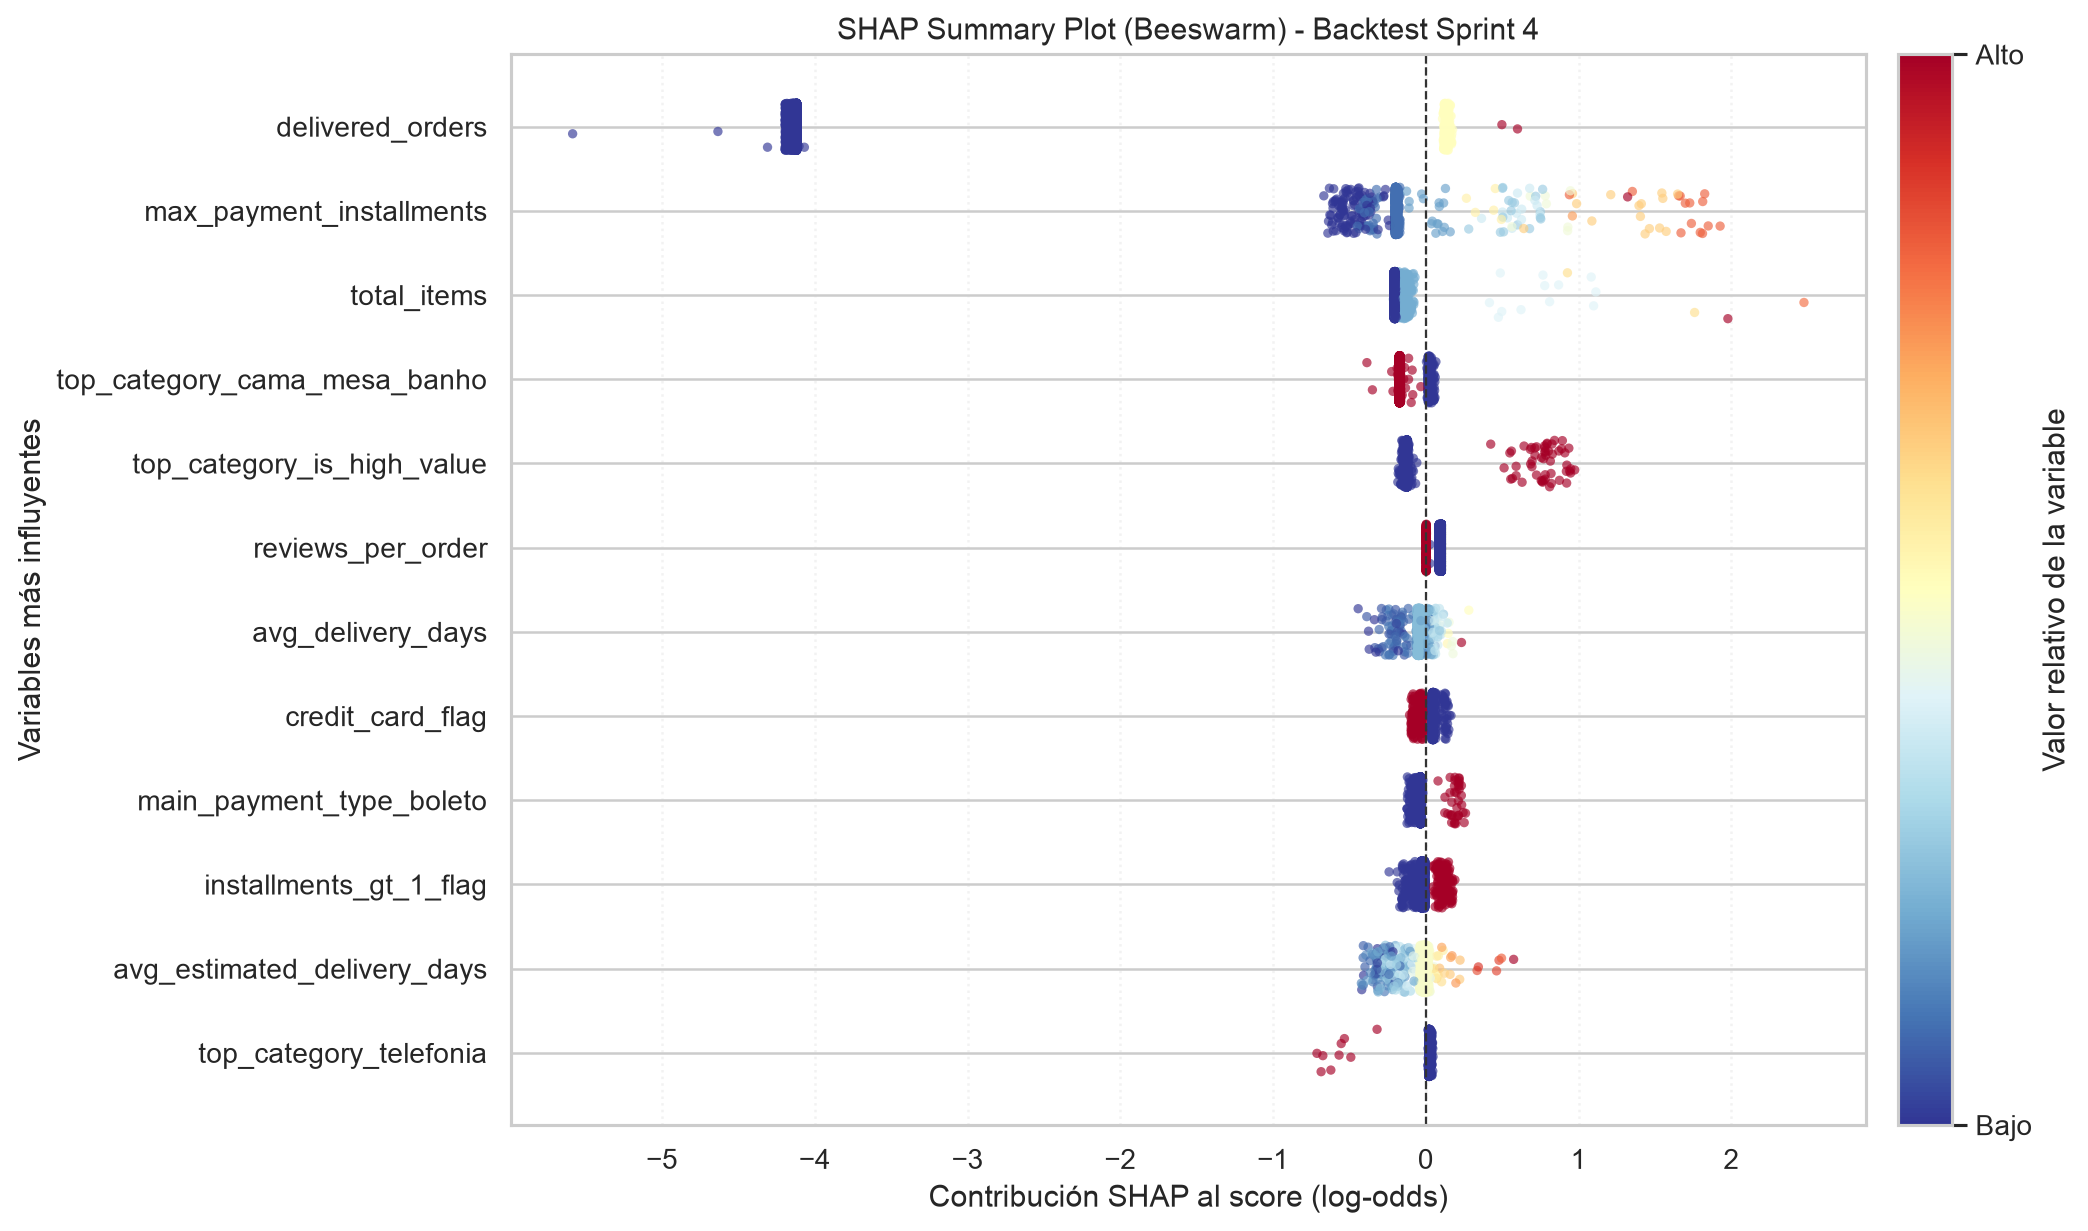
\includegraphics[width=0.82\textwidth]{sprint_04_shap_beeswarm.png}
    \caption{SHAP Summary Plot del modelo final. Las principales senales son transaccionales y de comportamiento comercial.}
    \label{fig:ext_shap}
\end{figure}

Esto refuerza que el modelo no es una caja negra opaca. La prediccion puede trazarse a variables que negocio entiende y puede discutir.

\section{Impacto de Negocio}
Para traducir el score a una decision comercial, se compararon dos estrategias:
\begin{enumerate}[label=\arabic*.]
    \item campana masiva sobre toda la base;
    \item campana focalizada sobre clientes con probabilidad $\geq 0.55$.
\end{enumerate}

\begin{table}[h]
\centering
\caption{Comparativa de Estrategias Comerciales}
\label{tab:ext_roi}
\begin{tabular}{lrr}
\toprule
Metrica & Masiva & Focalizada \\
\midrule
Clientes contactados & 96,096 & 1,605 \\
Costo de campana & BRL 1,441,440.00 & BRL 24,075.00 \\
Ingreso por conversiones & BRL 150,360.00 & BRL 84,360.00 \\
Utilidad neta & BRL -1,291,080.00 & BRL 60,285.00 \\
ROI & -89.57\% & +250.40\% \\
\bottomrule
\end{tabular}
\end{table}

El contraste es suficientemente fuerte como para argumentar valor de negocio del modelo. La estrategia focalizada reduce drasticamente el costo comercial y convierte una campana inviable en una accion con retorno positivo.

\section{Privacidad, Gobernanza y Uso Responsable}
El analisis etico del proyecto se centro en dos preguntas:
\begin{enumerate}[label=\arabic*.]
    \item si el modelo usa o no datos sensibles directos;
    \item si las variables que si retiene pueden generar sesgos operativos.
\end{enumerate}

El modelo final no entrena con identificadores directos como \texttt{customer\_unique\_id}, \texttt{customer\_city} o \texttt{customer\_zip\_code\_prefix}. Tampoco utiliza datos financieros sensibles directos como numeros de tarjeta o cuentas bancarias. Sin embargo, conserva variables como \texttt{customer\_state}, \texttt{main\_payment\_type} o \texttt{max\_payment\_installments}, que pueden actuar como proxies de desigualdad geografica o bancarizacion.

Por ello, la recomendacion de gobernanza es:
\begin{itemize}
    \item usar el score como apoyo a priorizacion comercial y no como criterio automatico unico;
    \item monitorear distribuciones por region y metodo de pago;
    \item minimizar exposicion de identificadores tecnicos;
    \item exigir cifrado y control de acceso si el MVP se operativiza en un contexto real.
\end{itemize}

\section{Monitoreo y Criterio de Reentrenamiento}
El modelo fue entrenado con historia y, por tanto, no debe asumirse valido indefinidamente. La utilidad futura depende de que la relacion entre comportamiento de compra, logistica, pagos y definicion del segmento premium permanezca estable.

Se recomienda monitorear:
\begin{itemize}
    \item desempeno discriminativo: ROC-AUC, Gini, Precision, Recall;
    \item impacto comercial: ROI de la campana focalizada;
    \item estabilidad poblacional: tasa premium predicha y volumen priorizado;
    \item drift de variables clave: \texttt{delivered\_orders}, \texttt{total\_items}, \texttt{max\_payment\_installments}, \texttt{customer\_state}, \texttt{top\_category\_is\_high\_value}.
\end{itemize}

El criterio recomendado no es reentrenar por calendario fijo, sino por evidencia. Una regla operativa inicial puede ser:
\begin{itemize}
    \item alerta amarilla si el Gini cae mas de 20\% respecto al baseline;
    \item alerta roja si ademas cae el ROI o cambia bruscamente la tasa premium predicha;
    \item revision obligatoria si varias variables dominantes muestran drift simultaneo.
\end{itemize}

Cuando se confirme degradacion, el nuevo entrenamiento debe hacerse sobre una ventana temporal nueva y completa, separada del periodo que entreno el artefacto vigente.

\section{Conclusiones}
El proyecto demostro que la identificacion de clientes premium en Olist es viable cuando se aborda con una arquitectura de datos y modelado coherente con la estructura real del negocio.

Las conclusiones principales son:
\begin{enumerate}[label=\arabic*.]
    \item El perfilado inicial mostro que la recurrencia no era la senal principal del valor premium, lo que obligo a abandonar una lectura simplista del RFM tradicional.
    \item La definicion del target mediante P80 congelado produjo un segmento estadistica y comercialmente defendible.
    \item La ingenieria de variables y el pipeline reproducible permitieron transformar un baseline casi aleatorio en un sistema predictivo util.
    \item LightGBM ofrecio la mejor combinacion de discriminacion, estabilidad y capacidad operativa.
    \item El MVP demostro que el modelo puede integrarse a una capa funcional con explicabilidad y simulacion de ROI.
    \item La sostenibilidad del modelo depende de monitoreo, gobernanza y reentrenamiento basado en evidencia, no en calendario.
\end{enumerate}

Como siguiente etapa natural, el proyecto podria evolucionar hacia:
\begin{itemize}
    \item monitoreo historico mensual en dashboard;
    \item validaciones temporales mas estrictas con ventanas completas;
    \item captura de ROI observado en operacion real;
    \item politicas mas formales de fairness, cifrado y auditoria.
\end{itemize}

\end{document}
